\documentclass[assign]{article}

\usepackage{graphicx}
\usepackage{amsmath,amssymb,amsthm} % define this before the line numbering.
\usepackage{color}
\usepackage{eso-pic}
\usepackage{bm}
\usepackage{caption}
\usepackage{epstopdf}
\usepackage{picins}
\usepackage[boxed]{algorithm2e}
\usepackage{url}
\usepackage{enumerate}
\usepackage{paralist}

% Declaring commonly used math operators
\DeclareMathOperator{\ddiag}{Diag}
\DeclareMathOperator{\rrank}{rank}
\DeclareMathOperator{\vvec}{vec}
\DeclareMathOperator{\tr}{tr}

\newcommand{\PhiB}{\mathbf{\Phi}}
\newcommand{\Ll}{\mathcal{L}}
\newcommand{\Nn}{\mathcal{N}}
\newcommand{\Uu}{\mathcal{U}}
\newcommand{\Ee}{\mathcal{E}}
\newcommand{\Aa}{\mathcal{A}}
\newcommand{\Hh}{\mathcal{H}}
\newcommand{\Ii}{\mathcal{I}}
\newcommand{\Ff}{\mathcal{F}}
\newcommand{\Dd}{\mathcal{D}}
\newcommand{\Tt}{\mathcal{T}}
\newcommand{\Pp}{\mathcal{P}}
\newcommand{\Ss}{\mathcal{S}}
\newcommand{\Cc}{\mathcal{C}}
\newcommand{\Oo}{\mathcal{O}}
\newcommand{\Bb}{\mathcal{B}}
\newcommand{\Rr}{\mathcal{R}}
\newcommand{\Rm}{\mathrm{R}}
\newcommand{\CB}{\mathbf{C}}
\newcommand{\RB}{\mathbf{R}}
\newcommand{\xB}{\mathbf{x}}
\newcommand{\yB}{\mathbf{y}}
\newcommand{\fB}{\mathbf{f}}
\newcommand{\ZB}{\mathbf{Z}}
\newcommand{\SB}{\mathbf{S}}
\newcommand{\AB}{\mathbf{A}}
\newcommand{\WB}{\mathbf{W}}
\newcommand{\TB}{\mathbf{T}}

\newcommand{\omitme}[1]{}
\newtheorem*{lemma}{Lemma}
\newtheorem{case}{Case}

\newenvironment{claim}[1]{\par\noindent\underline{{\bf Claim:}}\space#1}{}
\newenvironment{claimproof}[1]{\par\noindent\underline{{\bf Proof:}}\space#1}{\hfill$\square$}

\title{Homework 3}

\author{Prateep Mukherjee}

\begin{document}
\maketitle

\noindent 1. 
\par \noindent a)  A ``winning order" can be generated for a finite set of residents given the problem statement, can be proved through {\em principle of induction}. 

Let, $n$ denote the number of Pongville residents.

\textbf{Base case:} If $n=2$, the ``winning order" is the relative ordering of the two players. So, if $1^{st}$ player defeats $2^{nd}$, then the order is $(1 , 2)$, else
the order is $(2,1)$.  If $n = 3$, there are two possible scenarios. The two cases are shown in Fig. \ref{fig1}. (i) \textbf{Without cycle:} The order can be written as $(3 ,1 ,2)$, (ii) \textbf{With cycle:} The order can be written as $(3,1,2,3)$.

\parpic[r] {
\begin{minipage}{0.5\textwidth}
{
  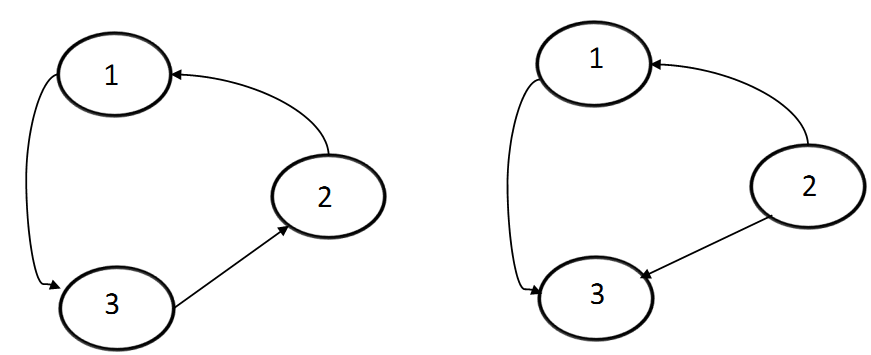
\includegraphics[width=\linewidth]{fig1.png}
   \captionof{figure}{The two scenarios. \textbf{Left} with cycle; \textbf{Right} without cycle.}
 \label{fig1}
  \vspace{-3pt}
}
\end{minipage}
}

\par\textbf{Inductive case:} Assume $n$ residents of Pongville has been arranged in the ``winning order''. Next we add another resident, say $A_{n+1}$ to the graph. Finally, we need to prove that the sequence generated from $n+1$ residents is also a ``winning order''.  There can be 3 different positions for $A_{n+1}$.

\begin{enumerate}[i]
  \addtolength{\itemsep}{-8pt}
  \item $A_{n+1}$ defeats everyone else. So, we can add $A_{n+1}$ to the end of the list. 
  \item $A_{n+1}$ loses to everyone else. So, we can add $A_{n+1}$ to the beginning of the list.
  \item $A_{n+1}$ wins some and loses some. In this case, we find a position, say $i$, in the existing order, such that player at $i-1$ loses to $A_{n+1}$ while that at $i+1$ wins the match against $A_{n+1}$. 
\end{enumerate}

\vspace{-5pt}
\noindent This completes the proof that a ``winning order'' can be generated given the graph. 
 
\par \noindent b) The algorithm to compute a ``winning order'' is designed as follows:

\fbox{
\begin{minipage}{0.95\linewidth}
\small {
  \begin{compactenum}[\bfseries {Step} 1:] 
    \item Compute the in-degree and out-degree of every vertex in $V$. Choose the vertex($u$) with maximum out-degree. Initialize $order = \phi$ 
    \item For each node $v \in N(u)$, if $v$ has not been visited, do one of the following. If: there exists edge $u \rightarrow v$ in G, append $v$ to the beginning of the list. Else: traverse the rest of  $order$ to find an appropriate(as discussed in (a)) place for inserting $v$. Goto step 1 and reiterate with $v$. 
    \item If no such $v$ exists, {\em terminate}, as we have reached the end of the sequence. 
   \end{compactenum}
}
\end{minipage}
}

\begin{proof}[\underline{\bf{Proof of correctness:}}] The graph G is a strongly connected graph. So, there is an edge between every pair of nodes. Therefore, one iteration over the set of nodes visits every node in the graph. Hence, our algorithm is guaranteed to generate an optimal ``winning order''. The algorithm has two nested loops, one for iterating over each vertex, and another for finding an appropriate position for it. Thus, the overall algorithm is $\Oo(V^2)$.
\end{proof}

\noindent 2. 
\par \noindent a) The given algorithm does not always compute a maximum flow. The latter can be proved if we can show that the algorithm fails to compute the maximum flow for any given graph(Proof by exception).

\begin{proof} 
\noindent An example is shown in Fig. \ref{fig2}. The maximum feasible flow computed using this algorithm on $G$ is 1.  

\begin{figure}[!hbt]
  \begin{center}
  \[\begin{array}{cccc}
  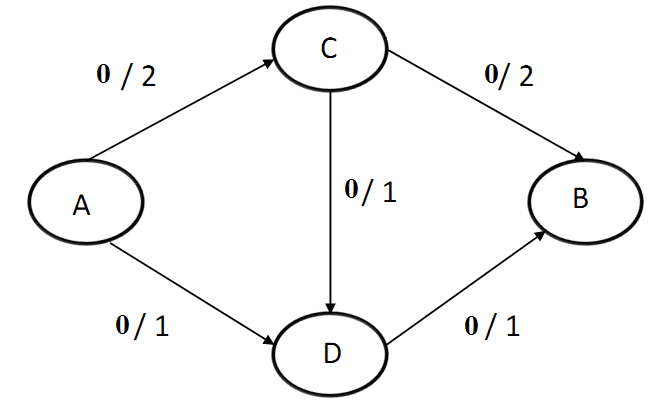
\includegraphics[width=0.29\linewidth] {fig2a.png} &
   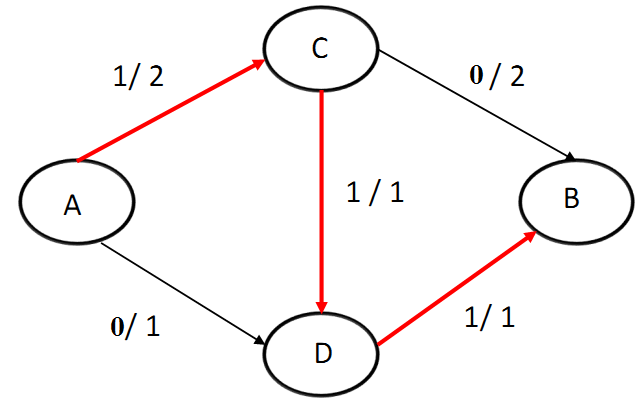
\includegraphics[width=0.29\linewidth] {fig2b.png} &
   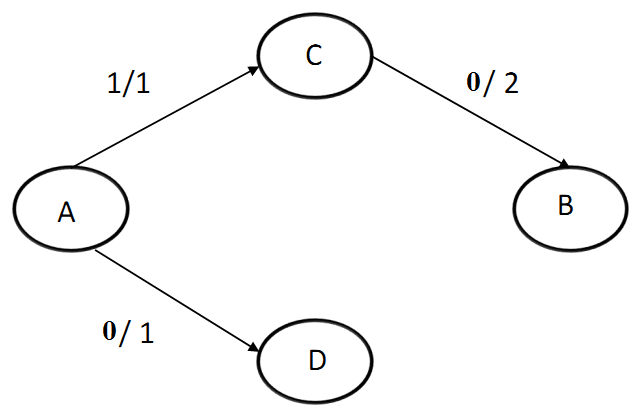
\includegraphics[width=0.29\linewidth] {fig2c.png} \\
 (a) & (b) & (c) \\
   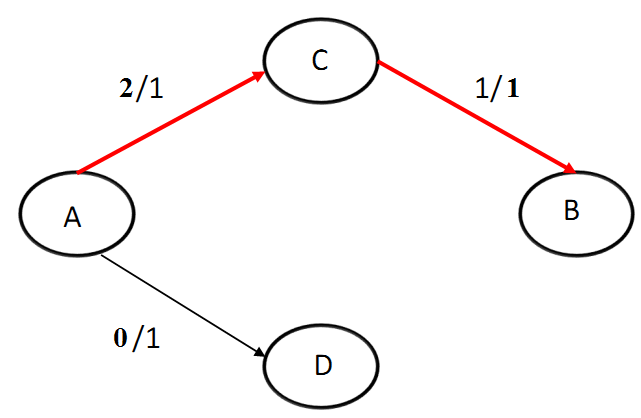
\includegraphics[width=0.29\linewidth] {fig2d.png} &
   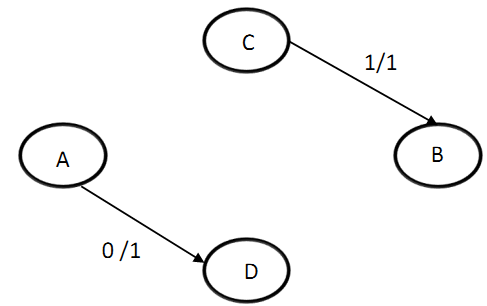
\includegraphics[width=0.29\linewidth] {fig2e.png} \\
 (d) & (e) \\
  \end{array}\]
\end{center}
\vspace{-5pt}
\caption{\small {One iteration of the algorithm is shown. Node $A$ is the source and $B$ is the target. \textbf{(a)} A graph $G=(V,E), V=\{A,B,C,D\}$ is shown with each edge $e$ labeled with flow($f$) / maximum capacity($c$); \textbf{(b)} A path $\pi$ is chosen(edges marked in red); \textbf{(c)} The residual graph shown after removing the edges; \textbf{(d)} Path $\pi$ is shown in red. Removing this path disconnects the graph \textbf{(e)} , therefore the algorithm terminates. 
}}
\label{fig2}
\end{figure}

\vspace{-10pt}
However, the maximum feasible flow in this graph is 3(2(AC), 0(CD), 1(AD),  2(CB), 1(DB)). Hence proved.
\end{proof}

\vspace{-5pt}
\par \noindent b) The maximum flow along $G$ can be computed using any maxflow algorithm, like {\em Ford-Fulkerson}. We can show that if the oracle picks a path from the set of augmenting paths used in the residual graph $G_f$ of the Ford-Fulkerson algorithm, at each iteration of the given algorithm, we can compute the optimum maximum flow.

\begin{proof}
     Let, $M$ be the set of augmenting paths from source to target.  The max-flow algorithm saturates an edge in each augmenting path in the residual graph $G_f$. So, if the oracle choses a path $p \in M$, saturating  $p$  and removing the saturated edge ensures a maximum flow along that path. Therefore, choosing the path $\pi$ from $M$ always guarantees an optimum maximum flow. Hence proved.
\end{proof}

\noindent 3. The problem statement can be restated as follows: Given a graph $G=(V,E)$, find the minimum number of vertices removing which disconnects the graph. This indicates a minimum cut solution to determine the minimum number of buildings in order to disconnect WEB \& ML. However, there are two requirements that are needed in order to apply a standard max-flow min-cut algorithm. 
\begin{compactenum}
  \item The graph $G$ must be directed acyclic.
  \item The min-cut algorithm will output the minimum number of edges to disconnect the graph, and not the minimum number of vertices.
\end{compactenum}

\noindent Note that the given graph in the problem is undirected. So, first we need to transform the undirected graph($G$) to a directed acyclic one($\tilde{G}=(\tilde{V},\tilde{E})$)). An easy solution to this is an undirected edge $(u - v)$ can be replaced by two directed edges $u \rightarrow v$ and $v \rightarrow u$.
\par\noindent The next step is to transform the goal from finding the minimum number of vertices to finding the minimum number of edges, so that a standard max-flow min-cut algorithm can be applied.  The solution here is split every vertex into two and introduce a ``fake'' directed edge($\tilde{e}$) between them, i.e. $\{\tilde{e} | \tilde{e} \in \tilde{E} \; \; \& \; \; \tilde{e} \notin E\}$. So, now the problem to finding the minimum set of vertices reduces to finding the minimum number of ``fake'' edges to disconnect the graph.

\vspace{-10pt}
\begin{figure}[!hbt]
\begin{center}
  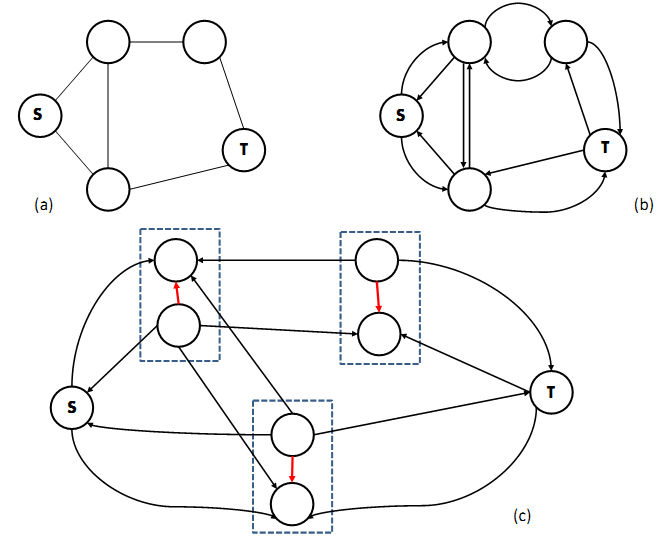
\includegraphics[width=0.78\linewidth]{fig3.png}
\end{center}
\caption{\small{ \textbf{(a)} original graph($G=(V,E)$); \textbf{(b)} the undirected graph converted to directed by introducing two directed edges for each edge;
\textbf{(c)} augmented directed graph $\tilde{G} = (\tilde{V}, \tilde{E})$, where $|\tilde{V}| = 2\times|V|$  and $|\tilde{E}| = 2\times|E| + |V|$. \textbf{S} represents WEB and \textbf{T} represents ML. ``Fake'' edges are denoted in \textcolor{red}{red}.
}}
\label{fig3}
\end{figure}

\par A transformation on a simple graph is shown in Fig. \ref{fig3}.  Each vertex($v$) is split into two vertices, namely \emph{in-vertex} and \emph{out-vertex}. All the incoming edges onto $v$ are directed to \emph{in-vertex}, while all the outgoing edges from $v$ are directed to \emph{out-vertex}. The ``fake edge'' for $v$ is directed from \emph{out-vertex} to \emph{in-vertex}, as shown in Fig. \ref{fig3}. To ensure that only ``fake'' edges are in the min-cuts, we make the capacities of ``real'' edges to be $\infty$, and that of ``fake'' edges to be 1. Now, we apply the Dinits algorithm(Short-pipes) to find the minimum cut. The capacities ensure that only the fake edges are cut. The number of edges in the minimum cut is equal to the minimum number of nodes to be disconnected. 
The time complexity of the algorithm is 
\begin{eqnarray*}
 \Oo(\tilde{V}\tilde{E}^2) &=& \Oo((2\times V) . (2\times E  + V)^2)  \\
                                      &=& \Oo(8\times VE^2 + 8\times EV^2 + 2\times V^3) \\
					 &=& \Oo(V^3 + VE^2).
\end{eqnarray*}

\begin{proof}[\underline{\textbf{Proof of correctness:}}]
   The graph $\tilde{G}$ is directed acyclic. Therefore, max-flow/min-cut algorithm successfully finds a minimum cut. Also, since capacities of real edges are $\infty$, they will never be saturated and thus not included in the minimum cut. Disconnecting the ``fake'' edges means removing the vertices. Therefore, the solution to the minimum cut problem is the optimum solution for our problem. Hence proved.
\end{proof}

\begin{figure}[!hbt]
\begin{center}
  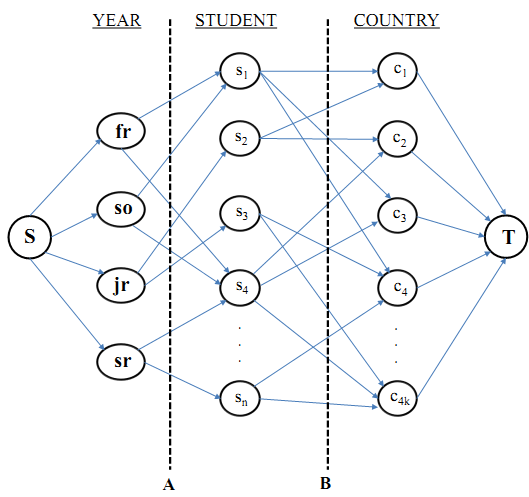
\includegraphics[width=0.9\linewidth]{fig4.png}
\end{center}
\vspace{-10pt}
  \caption{\small{ The maxflow graph $G$ is shown. $S$ is the source, $\{fr,so,jr,sr\}$ denotes the different years, $s_i$ are the students, $c_j$ are the countries, and $T$ is the sink/target. An edge $(s_i,c_j)$ indicates that student $s_i$ is affiliated with country $c_j$. The dotted lines \textbf{A} and \textbf{B} show the barriers across which flow is transfered. } }
  \label{fig4}
\end{figure}

\noindent 4. The given problem is modeled as a max-flow algorithm. The maxflow graph $G=(V,E)$ can be designed as shown in Fig \ref{fig4}. 

\noindent Now, the total number of countries is assumed to be $4k$.  Therefore, the total flow that crosses barrier \textbf{B} is at most $4k$. According to the \emph{conservation of flow} theorem, the total flow across barrier \textbf{A} is at most $4k$ too. The net outflow from the source $S$ to the first layer, therefore, is $4k$. Also according to the question, the committee will have equal number of freshmen, sophomore, junior and seniors. Hence, the capacity of each edge $(S \rightarrow y_i)$ is $k$, where $y_i$ denotes a node in the first layer.  The year-student and student-country edges are all of same capacity, as they are all of same priority. 
\par\noindent Each country can be represented by at most one student in the committee. Thus, the capacities of the edges in the final layer are also constant. Therefore,  if $f(e)$ and $c(e)$ represent the flow and capacities of edge $e \in E$ respectively, then the above problem can be mathematically formulated as follows:

\begin{equation}
\hspace{-50pt}
  \emph{maximize} \quad  f  \\
\label{eq1} 
\end{equation}
\begin{eqnarray*}
 s.t. \qquad \qquad f(e)  &\rightarrow& feasible \; flow, \quad \forall e \in E,  \\
  c(S,y_i) &=& k, \quad \forall y_i \in \{year\}  \\
  c(y_i,s_j) &=& 1, \quad \forall y_i \in \{year\}, s_j \in \{students\} \\
 c(s_i,c_j) &=& 1, \quad \forall s_i \in \{students\}, c_j  \in \{country\}  \\
 c(c_j,T) &=& 1, \quad \forall c_j \in \{country\}  \\
\end{eqnarray*}

Eq. \ref{eq1} can be solved using the standard algorithms for \emph{max-flow}. For this example, we can use \emph{Ford-Fulkerson} algorithm to obtain the maximum flow in $\Oo (E\fB)$, where $\fB$ is the maximum flow. 

\begin{proof}[\underline{\bf{Proof of correctness:}}] The capacities across the edges ensure that the maximum flow will guarantee optimal assignment of students to countries.  However, \textbf{one might be able to generate an example graph which has no possible solution.} For example, a country is affiliated by only one student while the latter has more than one affiliations, and the max-flow algorithm saturates an edge connecting  the student with some other country. In this case, the said country won't have a representative. Hence, the max-flow algorithm does not always generate a possible solution.
\end{proof}

\noindent 5.  The goal of this problem is to find the shortest path between {\em every} pair of vertices in a undirected weighted graph $G=(V,E,w), w: E \mapsto \Re$, such that the weight of the edges in that path is maximized. First, we define the value of a path between a pair of nodes. Let, $P = e_1e_2 \cdots e_k$ be a path between nodes $i$ \& $j$ ($i,j \in V$, $e_i \in E$). Value of the path P, denoted as V(P), is defined as :

\begin{equation}
  V(P) = \max_{i=[1,k], e_i \in P} w_{e_i} \notag
\end{equation} 

\noindent Thus, our problem is equivalent to find, for every pair of nodes $i$ and $j$, a minimum value path from node $i$ to $j$. Let, $T$ be the {\em minimum spanning tree}(MST) on G. 

\begin{claim}
  The unique path between nodes $i$ and $j$ in $T$ is the minimax path between them in G.
\end{claim}

\begin{claimproof}
   Let $P$ be the unique path between $i$ and $j$ in $T$. So, if $(v_k,v_l)$ is the maximum weight edge in the path $P$, removing $(v_k,v_l)$ from $T$ creates two partitions $S$ and $S'$, such that $i \in S$ and $j \in S'$. This defines a cut $(S,S')$.

 According to the {\em cut property}\footnote{Cut property: \url{http://en.wikipedia.org/wiki/Minimum_spanning_tree#Cut_property}} of a MST, for any edge $(i',j')$  such that $i' \in S$ and $j' \in S'$, $w_{v_k,v_l} \le w_{v_i',v_j'}$. 
\par Since any path $P'$ between $i$ and $j$ must contain all the nodes from the cut $(S,S')$, $w_{v_k,v_l}$ is the value of the path $P$, $P$ must be the minimum value path. This establishes that the unique path in MST $T$ is the minimax path between each pair of nodes in $G$. Extending this argument for all pairs of nodes in $G$ completes our proof. 
\end{claimproof}

\par The algorithm to compute the minimax path of $G$ hence consists of two steps: (i) Compute the MST T in G, (ii) return the unique path between every pair of nodes in T. The first step takes $\Oo(|E| \log |V|) = \Oo(|E| \log |E|)$ using Kruskal's algorithm. The second step is $\Oo(|E|)$ worst case. Thus, the total time complexity of our algorithm is $\Oo(|E| \log |E|)$.

\end{document}
